\usetikzlibrary{positioning,calc}
\graphicspath{ {../../images/} }

\title{ICS0026 Cryptography}
\subtitle{Secret sharing \& MPC}
\date{\today}
\author{Taaniel Kraavi}
\institute%
{%
  \textit{IT College}\\
  \textit{Tallinn University of Technology}
}

\begin{document}
\begin{frame}
  \titlepage
\end{frame}

\begin{frame}{Secrets and sharing}
  In symmetric schemes, a secret should be known by all participating parties.
  \begin{itemize}[<+(1)->]
    \item Shared secret: each party knows the same secret
    \item Can all these parties be trusted?
  \end{itemize}

  \vspace*{1em}

  \pause
  In asymmetric schemes, the secret is known by (usually) a single party.
  \begin{itemize}[<+(1)->]
    \item What if the party loses the secret?
  \end{itemize}

  \vspace*{1em}

  \pause
  Can we combine the trust and availability into a single scheme?
\end{frame}

\begin{frame}{Secret sharing}
  Split a secret into shares, and distribute them within a group.
  \begin{itemize}[<+(1)->]
    \item \emph{Players}: holders of the secret shares
    \begin{itemize}
      \item A trusted \emph{dealer} generates the secret and splits it among the players
    \end{itemize}
    \item \emph{Threshold}: minimum number of shares to reconstruct/use the secret
    \begin{itemize}
      \item e.g. nuclear launch codes/approval
    \end{itemize}
    \item $(t, n)$-threshold: $t$ out of $n$ players are needed to use the secret
    \begin{itemize}
      \item The subset of players matters not (good for availability)
    \end{itemize}
  \end{itemize}

  \vspace*{1em}

  \pause
  NB! Shared secret vs secret sharing: easy confusion!
  \begin{itemize}[<+(1)->]
    \item Shared secret: everyone has the same secret
  \end{itemize}
\end{frame}

\begin{frame}{Secure secret sharing}
  We will focus only on \emph{secure} secret sharing schemes
  \begin{itemize}[<+(1)->]
    \item No info is leaked by obtaining less than $t$ shares
    \begin{itemize}
      \item Knowing $<t$ shares $\iff$ knowing $0$ shares
    \end{itemize}
    \item Insecure schemes exist
    \begin{itemize}
      \item e.g. naive string splitting
    \end{itemize}
  \end{itemize}

  \vspace*{1em}

  \pause
  Is the nuclear launch-code splitting secure or insecure?
\end{frame}

\begin{frame}{How many to corrupt?}
  Confidentiality
  \begin{itemize}[<+(1)->]
    \item Corrupt $t$ players to breach secrecy
  \end{itemize}

  \vspace*{1em}

  \pause
  Integrity \& availability
  \begin{itemize}[<+(1)->]
    \item Corrupt $n - t + 1$ players to completely destroy/alter the secret
  \end{itemize}

  \vspace*{1em}

  \pause
  What should $t$ be to ensure the will of the majority?
\end{frame}

\begin{frame}{Some special cases}
  As a warm-up, how can we solve the following?
  \begin{itemize}[<+(1)->]
    \item $t = 1$
    \item $t = n$
  \end{itemize}

  \vspace*{1em}

  \pause
  Suppose now that an efficient scheme for $1 < t < n$ exists.
  \begin{itemize}
    \pause \item How to have different decision \enquote{powers}?
    \begin{itemize}
      \pause \item CEO can do whatever
      \item The rest of C-suite needs to collaborate
    \end{itemize}
  \end{itemize}

  \vspace*{1em}

  \pause
  The tricky part: how to design an efficient $1 < t < n$ scheme?
\end{frame}

\begin{frame}{A geometric approach}
  $n+1$ non-parallel $n$-dimensional hyperplanes \emph{can} intersect at a unique point\textsuperscript{*}.
  \begin{itemize}[<+(1)->]
    \item Two non-parallel lines intersect at a unique point
    \item Three pairwise non-parallel planes \emph{can} intersect at a unique point
    \pause
    \vspace*{1em}
    % https://tex.stackexchange.com/a/45249
    \begin{figure}
      \centering
      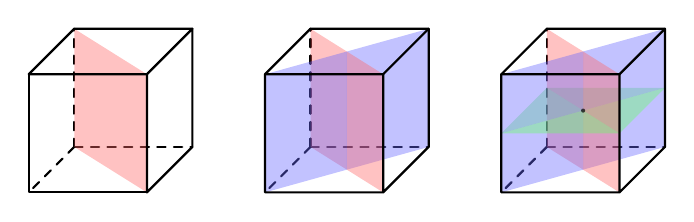
\begin{tikzpicture}[scale=1.5,fill opacity=0.4,thick,
        line cap=round,line join=round]
        %% Define coordinate labels.
        % t(op) and b(ottom) layers
        \path \foreach \layer/\direction in {b/{0,0,0},t/{0,1,0}} {
          (\direction)
          \foreach \point/\label in {{0,0,0}/ll,{1,0,0}/lr,{1,0,-1}/ur,{0,0,-1}/ul} {
            +(\point) coordinate (\layer\label)
          }
          ($(\layer ll)!0.5!(\layer ur)$) coordinate (\layer md)
        };
    
        % Draw left cube.
        \foreach \direction in {(0,0,1),(0,1,0),(1,0,0)} {
          \draw[dashed] (bul) -- + \direction;
        }
        %\fill[blue!60] (bmd) -- (bur) -- (tur) -- (tmd);
        \fill[red!60]  (blr) -- (tlr) -- (tul) -- (bul);
        %\fill[blue!60] (bll) -- (bmd) -- (tmd) -- (tll);
        \draw (bll) -- (blr) -- (tlr) -- (tll) -- cycle;
        \draw (blr) -- (bur) -- (tur) -- (tlr) -- cycle;
        \draw (tll) -- (tlr) -- (tur) -- (tul) -- cycle;
    
        % Draw middle cube.
        \path (blr) + (1,0) coordinate (pos);
        \foreach \direction in {(0,0,1),(0,1,0),(1,0,0)} {
          \draw[dashed] (pos) ++ (bul) -- + \direction;
        }
        \fill[blue!60] (pos) +(bmd) -- +(bur) -- +(tur) -- +(tmd);
        \fill[red!60]  (pos) +(blr) -- +(tlr) -- +(tul) -- +(bul);
        \fill[blue!60] (pos) +(bll) -- +(bmd) -- +(tmd) -- +(tll);
        \draw (pos) +(tll) -- +(tlr) -- +(tur) -- +(tul) -- cycle;
        \draw (pos) +(tll) -- +(bll) -- +(blr) -- +(bur) -- +(tur) +(blr) -- +(tlr);

        % Draw right cube.
        \path (pos) + (2,0) coordinate (pos2);
        \foreach \direction in {(0,0,1),(0,1,0),(1,0,0)} {
          \draw[dashed] (pos2) ++ (bul) -- + \direction;
        }
        \fill[green!60] (pos2) +(0, 0.5, -1) -- +(0.5, 0.5, -0.5) -- +(1, 0.5, -1) -- +(0, 0.5, -1);
        \fill[blue!60] (pos2) +(bmd) -- +(bur) -- +(tur) -- +(tmd);
        \fill[green!60] (pos2) +(1, 0.5, 0) -- +(0.5, 0.5, -0.5) -- +(1, 0.5, -1) -- +(1, 0.5, 0);
        \fill[red!60]  (pos2) +(blr) -- +(tlr) -- +(tul) -- +(bul);
        \fill[green!60] (pos2) +(0, 0.5, 0) -- +(0, 0.5, -1) -- +(0.5, 0.5, -0.5) -- +(0, 0.5, 0);
        \fill[blue!60] (pos2) +(bll) -- +(bmd) -- +(tmd) -- +(tll);
        \fill[green!60] (pos2) +(0, 0.5, 0) -- +(0.5, 0.5, -0.5) -- +(1, 0.5, 0) -- +(0, 0.5, 0);
        \draw (pos2) +(tll) -- +(tlr) -- +(tur) -- +(tul) -- cycle;
        \draw (pos2) +(tll) -- +(bll) -- +(blr) -- +(bur) -- +(tur) +(blr) -- +(tlr);
        \fill[fill opacity=0.7] (pos2) +(0.5, 0.5, -0.5) circle (0.5pt);
      \end{tikzpicture}
    \end{figure}
    \item \dots
  \end{itemize}

  \vspace*{1em}

  \pause
  Blakley's scheme is based on this approach.
\end{frame}

\begin{frame}{Polynomial interpolation}
  Given $n+1$ distinct points, there is a unique polynomial of degree at most $n$ that passes through these points.
  \begin{itemize}[<+(1)->]
    \item Two distinct points define a line
    \item Three distinct points define a quadratic function
    \begin{itemize}
      \item If the points are aligned, the result is a line, i.e. $a=0$
    \end{itemize}
    \item \dots
  \end{itemize}

  \vspace*{1em}

  \pause
  Polynomial interpolation is a procedure to find such a polynomial.

  \pause
  Lagrange interpolating polynomial:
  \begin{itemize}
    \item Polynomial of lowest degree that interpolates a given set of points
  \end{itemize}
\end{frame}

\begin{frame}{Shamir's secret sharing}
  Shamir's secret sharing is based on polynomial interpolation over finite fields.
  \begin{enumerate}[<+(1)->]
    \item Pick a secret integer $a_0 \getsu \ZZ_q$
    \item Randomly pick $t-1$ elements $a_1, \dots, a_{t-1}$ from $\ZZ_q$
    \item Construct the polynomial of degree $t-1$
    \[
      f(x) = a_0 + a_1 x + a_2 x^2 + \dots + a_{t-1} x^{t-1} \pmod{q}
    \]
    \item Compute $n$ secret shares
    \begin{itemize}
      \item For $i=1, \dots, n$ the $i$-th secret share is the point $(i, f(i))$
      \item Give $(i, f(i))$ to the $i$-th player
      \item $i$ can be made public, but $f(i)$ must be secret
    \end{itemize}
  \end{enumerate}

  \pause
  To recover the secret, find the Lagrange polynomial and compute $f(0)$.
\end{frame}

\begin{frame}{Issues with Shamir}
  Secret sharing is not verifiable:
  \begin{itemize}[<+(1)->]
    \item A malicious party can submit a fake share
  \end{itemize}

  \pause
  There is a single point of failure:
  \begin{itemize}[<+(1)->]
    \item Need for a trusted dealer
    \item The secret exists in its entirety and can be stolen
    \begin{itemize}
      \item During generation and reassembly
      \item The shares must be directly available (knowledge and not possession)
    \end{itemize}
  \end{itemize}
\end{frame}

\begin{frame}{Solutions pt. 1}
  (Publicly) verifiable secret sharing
  \begin{itemize}[<+(1)->]
    \item Players can verify that shares are consistent
    \begin{itemize}
      \item Both during the dealing phase (malicious dealer) and reconstruction phase (malicious players)
    \end{itemize}
    \item Publicly verifiable if anyone can verify that participants received correct shares (players have public keys)
    \item We will not go into the maths here
    \begin{itemize}
      \item Benaloh's scheme, Feldman's scheme, Pedersen's scheme, \dots
    \end{itemize}
  \end{itemize}
\end{frame}

\begin{frame}{Solutions pt. 2}
  Distributed share generation \& multiparty computation (MPC)
  \begin{itemize}[<+(1)->]
    \item Players (verifiably) generate their own shares
    \begin{itemize}
      \item Pairs well with crypto hardware, e.g. JavaCards
    \end{itemize}
    \item The public key is constructed from public data output by the players
    \item The secret key is never reconstructed
    \begin{itemize}
      \item $t$ players must perform partial operations on the data instead
    \end{itemize}
    \item The partial data are then combined to obtain the full result
    \item An approachable example:
    \begin{itemize}
      \item \href{https://link.springer.com/chapter/10.1007/3-540-46416-6_47}{\textit{A Threshold Cryptosystem without a Trusted Party}} by Torben Pedersen
    \end{itemize}
  \end{itemize}
\end{frame}

\begin{frame}{Secure multi-party computation}
  Secure multi-party computation (MPC) is needed to jointly compute a function over private inputs.
  \begin{itemize}[<+(1)->]
    \item Privacy between participants, and not just against outsiders
    \item E.g. Yao's millionaires' problem
    \begin{itemize}
      \item Two millionaires attempt to determine which of the two is richer
      \item They do not want to reveal their wealth while doing so
    \end{itemize}
  \end{itemize}

  \pause
  Two core properties:
  \begin{itemize}[<+(1)->]
    \item Input privacy
    \item Correctness of computation
  \end{itemize}
\end{frame}

\begin{frame}{Approaches to MPC}
  Commonly, MPC is based on secret sharing and boolean or arithmetic circuits.
  \begin{itemize}[<+(1)->]
    \item Fully homomorphic encryption can be used to perform MPC
    \item Zero knowledge proofs can be used in, for, or with with MPC
    \item In general, MPC protocols can get very complex and are out of our scope
    \begin{itemize}
      \item MPC alliance \href{https://wiki.mpcalliance.org/protocols.html}{\textit{wiki}}
    \end{itemize}
  \end{itemize}

  \vspace*{1em}

  \pause
  Some examples of MPC:
  \begin{itemize}[<+(1)->]
    \item Threshold signatures/threshold decryption
    \item Private information retrieval (PIR) / oblivious transfer (OT)
    \item Private bidding (notable mention: Danish Sugar Beet auction of 2008)
  \end{itemize}
\end{frame}

\begin{frame}{Secure AND}
  \pause
  The Tinder problem: how can two people decide whether they want to go out?
  \begin{itemize}[<+(1)->]
    \item If both are interested, the protocol should output $1$
    \item Otherwise, the protocol should output $0$
    \begin{itemize}
      \item A refusing party should not learn whether the other wanted the date
    \end{itemize}
  \end{itemize}

  \vspace*{1em}

  \pause
  The protocol is drawn on the whiteboard.
\end{frame}

\begin{frame}{Secret sharing (again)}
  Let us secretly share some integer $x$ between two parties $P_1, P_2$:
  \begin{itemize}[<+(1)->]
    \item We pick $x_1 \getsu \ZZ_q$, compute $x_2 \gets x - x_1$ and send $x_i$ to $P_i$
    \item Neither party knows anything about $x$, and we write $[x]$
    \item If the parties corroborate, they can recover $x$
    \begin{itemize}
      \item This is called \emph{opening} $[x]$
    \end{itemize}
  \end{itemize}
\end{frame}

\begin{frame}{Some computations}
  Let $[x]$ and $[y]$ be secret shared between $P_1, P_2$, and let $a$ be known to both.
  \begin{itemize}[<+(1)->]
    \item $[x + y]$
    \begin{itemize}
      \item $P_i$ computes $z_i \gets x_i + y_i$
      \item $P_1$ and $P_2$ can collaborate to get $z_1 + z_2 = x_1 + x_2 + y_1 + y_2 = x + y$
    \end{itemize}
    \item $[ax]$
    \begin{itemize}
      \item $P_i$ computes $w_i \gets ax_i$
      \item $P_1$ and $P_2$ can collaborate to get $w_1 + w_2 = ax_1 + ax_2 = a(x_1 + x_2) = ax$
    \end{itemize}
    \item $[x + a]$
    \begin{itemize}
      \item $P_1$ computes $u_1 \gets x_1 + a$ and $P_2$ computes $u_2 \gets x_2$
      \item $P_1$ and $P_2$ can collaborate to get $u_1 + u_2 = x_1 + a + x_2 = x + a$
    \end{itemize}
  \end{itemize}
\end{frame}

\begin{frame}{Difficulty of multiplication}
  We have shown how to obtain $x + y$, $ax$ and $x + a$ with MPC.
  \begin{itemize}[<+(1)->]
    \item How can we compute $[xy]$?
  \end{itemize}
\end{frame}

\begin{frame}{Beaver triples}
  Let a dealer pick $a, b \getsu \ZZ_q$ and secret share $[a], [b], [a \cdot b]$ with $P_1, P_2$.
  \begin{enumerate}[<+(1)->]
    \item Both parties compute and open $[x + a]$ and $[y + b]$.
    \begin{itemize}
      \item It is okay to open them since $a$ (resp. $b$) perfectly masks $x$ (resp. $y$).
    \end{itemize}
    \item Both parties compute
    \begin{align*}
      &[x](y + b) + [y](x + a) - (x+a)(y+b) + [a\cdot b]\\
      &= [xy + xb + xy + ay - xy - xb - ay - ab + ab]\\
      &= [xy]
    \end{align*}
  \end{enumerate}
  \vspace*{-1em}
  \pause
  $([a], [b], [a \cdot b])$ is a Beaver triple.
  \begin{itemize}[<+(1)->]
    \item Can only be used once, otherwise information is leaked
    \item The triple is \emph{consumed} after use
  \end{itemize}
\end{frame}

\begin{frame}{Cybernetica coolness}
  Cybernetica has developed the \href{https://sharemind.cyber.ee}{\textit{Sharemind}} platform which uses MPC.
  \begin{itemize}[<+(1)->]
    \item Brainchild of Dan Bogdanov
    \item Used for privacy-preserving data analytics
    \item Runs on distributed non-colluding servers
    \item Pilot runs have been conducted in Estonia
    \begin{itemize}
      \item Are working IT students less likely to graduate? (2013--2015)
      \item Regulation did not allow for direct analysis of data: education vs tax records
      \item Sharemind was therefore used 
      \item No correlation was found
    \end{itemize}
  \end{itemize}
\end{frame}

\begin{frame}{Disclaimer}
  MPC and its threat models can get very complicated!
  \pause
  \begin{itemize}
    \item Active vs passive adversaries
    \item Number of corrupted parties
    \item Type of security guarantees (computational, statistical, perfect)
    \item Output guarantees, e.g. fairness, security with aborts
    \item \dots
  \end{itemize}

  \pause
  We did not even scratch the surface.
\end{frame}

\end{document}
